\documentclass[twoside,11pt]{article}

% Any additional packages needed should be included after jmlr2e.
% Note that jmlr2e.sty includes epsfig, amssymb, natbib and graphicx,
% and defines many common macros, such as 'proof' and 'example'.
%
% It also sets the bibliographystyle to plainnat; for more information on
% natbib citation styles, see the natbib documentation, a copy of which
% is archived at http://www.jmlr.org/format/natbib.pdf

\usepackage{jmlr2e}
\usepackage{multirow}
\usepackage{booktabs}
\usepackage{xspace}
\usepackage[table]{xcolor}
\usepackage{graphicx}
\usepackage[inline]{enumitem}
% \usepackage{siunitx}
% Definitions of handy macros can go here

\newcommand{\dataset}{{\cal D}}
\newcommand{\fracpartial}[2]{\frac{\partial #1}{\partial  #2}}

\newcommand{\ade}{\texttt{Adenine}\@\xspace}
\newcommand{\py}{\texttt{Python}\@\xspace}
\newcommand*{\ie}{i.e.\@\xspace}
\newcommand*{\eg}{e.g.\@\xspace}
\newcommand{\todo}[1]{\textcolor{red}{{\bf \{#1\}}}} %TODO

% Heading arguments are {volume}{year}{pages}{submitted}{published}{author-full-names}
\jmlrheading{X}{2016}{X-XX}{X/XX}{XX/XX}{Samuele Fiorini, Federico Tomasi and Annalisa Barla}

% Short headings should be running head and authors last names

\ShortHeadings{ADENINE}{Fiorini, Tomasi, Barla}
\firstpageno{1}

\begin{document}

\title{ADENINE --- A Data ExploratioN pIpeliNE}

\author{\name{Samuele Fiorini} \email{samuele.fiorini@dibris.unige.it}\\
\name{Federico Tomasi} \email{federico.tomasi@dibris.unige.it}\\
\name{Annalisa Barla} \email{annalisa.barla@unige.it}\\[1em]
\addr Department of Informatics, Bioengineering, \\Robotics and System Engineering (DIBRIS)\\
     University of Genoa\\
     Genoa, I-16146, Italy}


\editor{Editor name}

\maketitle

\begin{abstract}

In this paper we introduce \ade, a \py framework for data exploration. The main goal of \ade, is twofold: helping researchers and data scientists achieving a first and quick overview on the main structures underlying their data and choosing the most suitable unsupervised learning pipeline for the problem at hand. This software tool encompasses state of the art techniques for: missing values imputing, preprocessing, dimensionality reduction and clustering tasks.
\ade exploits both process and thread level parallelism and it is capable of generating nice and clean publication-ready figures along with quantitative descriptions of the pipelines performance. \ade is released under FreeBSD license and it can be downloaded from \href{http://slipguru.github.io/adenine/}{http://slipguru.github.io/adenine/}.


\end{abstract}

\begin{keywords}
Data exploration, unsupervised learning, RNA-Seq gene expression
\end{keywords}

\section{Introduction}\label{sec:intro}
Data exploration can be an extremely helpful starting point for many data analysis tasks. Researchers and data scientists are often asked to extract meaningful information from collections of complex and possibly high-dimensional data coming from heterogenous contexts. For instance, in biomedical scenarios, physicians are likely to be interested in answering some biological questions starting from a set of observations collected from a pool of subjects enrolled in a study. Possible investigations can be: \emph{is there any relevant stratification among subjects?} or \emph{is it possible to discriminate between cases and controls from my observations?}. Starting from a given dataset, the information needed to answer such questions may be immediate, non-trivial to extract or even completely absent.
In these situations, a preliminary data exploration step can be not only good practice, but also a mandatory starting point for further investigations. In this context, several machine learning and data mining techniques were developed over the years. Among those we focus on the four most popular families: \begin{enumerate*}[label=(\roman*)]
  \item missing values imputing,
  \item data preprocessing,
  \item dimensionality reduction and
  \item unsupervised clustering
\end{enumerate*}.

In the last few years, a fair number of data exploration software tools and libraries  were released. At a very coarse grain we can group them into two sets: interactive GUI-based and non-interactive script-based  applications. Of the first group, we recall \emph{Divvy} \citep{lewis2013divvy}, a software tool that performs dimensionality reduction and clustering on input datasets. \emph{Divvy} is a light framework, although it is only Mac OS X specific, it heavily lacks in documentation, its collection of \texttt{C/C++} algorithm implementations does not cover common strategies such as Kernel Principal Component Analysis (KPCA) \citep{scholkopf1997kernel} or Hierarchical Clustering \citep{friedman2001elements} and it does not offer strategies to perform automatic discoveries of the number of clusters. The most notable project that spans between the two families is \emph{Orange} \citep{demvsar2013orange}, a data mining software suite that offers both visual programming front-end and standard \py APIs. In the context of data exploration, \emph{Orange} can be successfully employed. However it does not support automatic pipeline generation, hence it requires the user to manually create each pipeline. On the other hand, as of today \emph{Orange} lacks in several nonlinear methods such as Spectral Embedding \citep{ng2002spectral}, Locally Linear Embedding \citep{roweis2000nonlinear} and Spectral Clustering \citep{shi2000normalized}.

We introduce \ade, a script-based \py tool for data exploration that, starting from a set of predefined unsupervised algorithms, creates textual an graphical reports of an arbitrary number of pipelines. In this context data imputing, preprocessing, dimenionality reduction and clustering strategies are considered as pipeline building blocks. The user is only required to specify the input data and which blocks should be activated and \ade takes care of automatically generate and run the pipelines made by all possible combinations of the selected algorithms. All \ade algorithm implementation is inherited, or extended, from \texttt{scikit-learn} \citep{scikit-learn} which is, to the best of our knowledge, the most complete machine learning open source library freely available online.

\section{Implementation}\label{sec:implem}
From an implemetative standpoint, \ade is built around the concept of \emph{pipeline}, that is a sequence of four fundamental steps:
\begin{enumerate*}[label=(\roman*)]
  \item missing values imputing,
  \item data preprocessing,
  \item dimensionality reduction and
  \item clustering
\end{enumerate*} (see Figure~\ref{fig:workflow}).

\begin{figure}[h!]
    \centering
    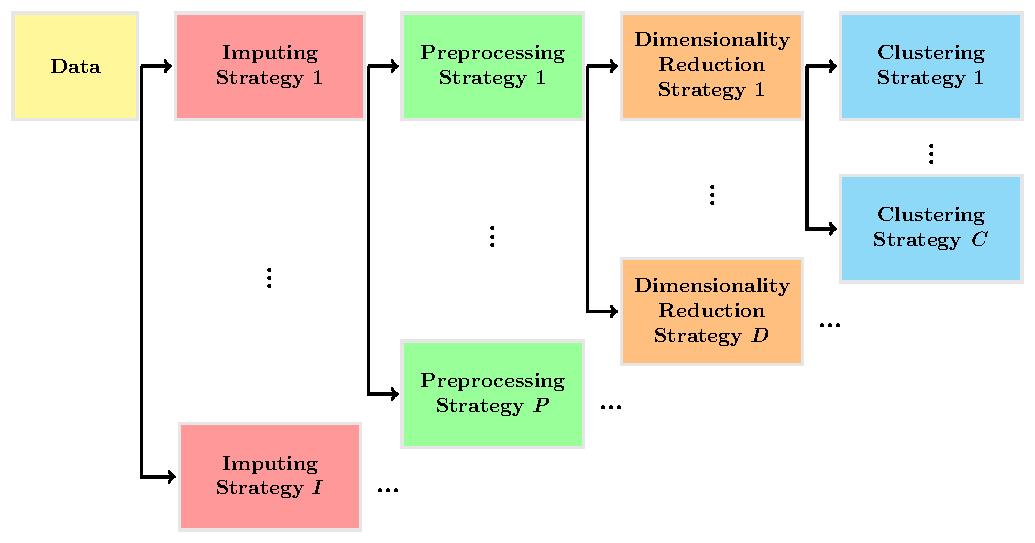
\includegraphics[width=\textwidth]{ade_wf/ade_wf.pdf}
    \caption{A schematic representation of the \ade workflow. The list of building blocks available for each step is summarized in Table~\ref{tab:blocks}.}\label{fig:workflow}
\end{figure}

For each step, a fair number of off-the-shelf algorithms are available (see Table~\ref{sec:implem}).

% For the first step, \ade offers an extended version of the \texttt{sklearn.preprocessing.Imputer} class that adds the \emph{KNN} imputing method to the pre-existent features-wise \emph{mean}, \emph{median} and \emph{most frequent} choices.

In order to perform exploratory analysis of large datasets, \ade can take advantage of different parallel computing paradigms. For instance, its pipelines are designed to be independent from each other, therefore they all run in parallel as separate \py processes on different cores. Moreover, since \ade makes large use of \texttt{numpy} and \texttt{scipy}, it automatically benefits from their bindings with optimized linear algebra libraries (such as OpenBLAS\footnote{\href{http://www.openblas.net/}{http://www.openblas.net/}}, or Intel\textsuperscript{\textregistered}~MKL).

\section{Experiments and results}
To assess the quality of the obtained results, we tested \ade on a set of synthetic and real dataset.

\todo{parla qui dei test synth}
\todo{TGCA}

\section{Conclusions}



%%%%%%%%%%%%%%%%%%%%%%%%%%%%%%%%%%%%%%%%%%%%%%%%%%%%%%%%%%%%%%%%%%%%%%%%%%%%%%%%%%%

\begin{table}[hbtp]
  {\caption{Pipelines building blocks and relative references (which are not reported when the definition is given in Section~\ref{sec:implem}).}\label{tab:blocks}}

  {\begin{tabular}{lll}
  \toprule
  \bfseries Step &   \bfseries Algorithms & \bfseries Ref.\\

  \multirow{2}{*}{Imputing} & Mean &  \\
  & Median & \\
  & KNN & \citep{troyanskaya2001missing} \\
  \midrule

  \multirow{4}{*}{Preprocessing} & Recentering &  \\
  & Standardize &  \\
  & Normalize &  \\
  & MinMax &  \\
  \midrule

  \multirow{9}{*}{\begin{tabular}{@{}c@{}}Dimensionality \\ reduction\end{tabular}} & Principal component Analysis (PCA) & \citep{jolliffe2002principal} \\
  & Incremental PCA & \citep{ross2008incremental} \\
  & Randomized PCA & \citep{halko2011finding} \\
  & Kernel PCA & \citep{scholkopf1997kernel} \\
  & Isomap & \citep{tenenbaum2000global} \\
  & Locally Linear Embedding & \citep{roweis2000nonlinear} \\
  & Spectral Embedding & \citep{ng2002spectral} \\
  & Multidimensional Scaling & \citep{borg2005modern} \\
  & \begin{tabular}{@{}l@{}}t-Distributed Stochastic \\ Neighbor Embedding (t-SNE)\end{tabular}   & \citep{van2008visualizing} \\
  \midrule

  \multirow{5}{*}{Clustering} & K-means &  \citep{bishop2006pattern}\\
  & Affinity propagation & \citep{frey2007clustering} \\
  & Mean Shift & \citep{comaniciu2002mean} \\
  & Spectral & \citep{shi2000normalized} \\
  & Hierarchical & \citep{friedman2001elements} \\

  \bottomrule
  \end{tabular}}
\end{table}

% \acks{Acknowledgements go here.}

\vskip 0.2in
\bibliography{adenine}

\end{document}
